\chapter{Finanzinstitute, Innovation und Regulatorik}
\label{ch:background}
Das nachfolgende Kapitel untersucht mithilfe einer Fallstudie die Auswirkungen von innovativen Technologien und Veränderungen auf das Finanzwesen. Sie enthält die wesentlichen Schritte aus \emph{Design-Thinking} für eine innovative Lösungsfindung, die mit dem Schritt \emph{emphatize} beginnt. Zudem betrachtet sie die Regulatorik und analysiert die Rahmenbedingungen.
\medskip
\\
Dazu beschäftigt sie sich mit den Rahmenbedingungen für Veränderungen in Kreditinstituten aus verschiedenen Perspektiven und betrachtet dabei die möglichen Einschränkungen und antreibenden Faktoren für die an verschiedenen Stellen bekannten Probleme in der IT-Architektur von Banken. Hierin werden auch die Auswirkungen der Regulatorik des Finanzwesens bezüglich der Maßnahmen für die IT untersucht.

\section{Transformation von Goldman Sachs}
\label{section:Goldman}
Goldman Sachs sieht sich nicht als Finanzdienstleister, sondern als ein Technologieunternehmen und als eine Plattform \cite{Gupta:2017}. Diese Transformation könnte als Vorbild für Institute des deutschen Finanzwesens dienen und eventuell wiederverwendbare Lösungen bieten.
\medskip
\\
Auf der einen Seite stehen die FinTechs, die sich Marktanteile im Privatkundenbereich sichern und zunehmenden Druck auf die etablierten Institute ausüben (\ref{Disruption:FinTechs}). Auf der anderen Seite richten sich anpassungsfähige Institute neu aus und etablieren sich mit Technologien und Plattformen in neue Geschäftsmodelle. 
\medskip
\\
Eines dieser Institute ist Goldman Sachs.
Gupta und Simonds \cite{Gupta:2017} haben die Transformation von Goldman Sachs hin zum selbsternannten Technologieunternehmen \cite{Gupta:2017} beschrieben. Nachfolgend werden die relevanten Punkte aus dieser Studie untersucht.
%
\paragraph{Auswirkung von Technologien auf Goldman Sachs}
 zu betrachten wie Goldman Sachs neue Technologien wahrnimmt und 

Folgende Auswirkungen ergaben sich durch neue Technologien für Goldman Sachs und waren ein Impuls für Veränderung \cite{Gupta:2017}:
\begin{itemize}
    \item Daten und Metriken wurden wertvoller als die Instinkte der Händler.
    \item Die Auswirkung von Technologie im Finanzwesen verstärkte sich seit der Finanzkrise 2008 umso stärker
    \item Cloud, Open-Source Software und Schnittstellen führten zu einer erheblichen Reduzierung von Zeit und Kosten in der eigenen Entwicklung von Technologien
    \item Verstärkter Wettbewerb durch FinTechs
\end{itemize}

Ein wichtiger Punkt für Goldman Sachs ist hierbei die Reduktion der Kosten für die eigene Entwicklung von Technologien. Verwendung von Open-Source oder Standardsoftware reduziert die Komplexität der IT-Architektur \cite{Bussmann2006}. Sie bringt die \ac{SEU} auf einen gemeinsamen Nenner und reduziert die Kosten. 

Mit der Verwendung von Open-Source Software für die Entwicklung von Anwendungen können gängige Lösungen einem individuellen Bedarf angepasst und verwendet werden. Hierdurch könnte sehr viel Aufwand in der Entwicklung eines eigenen Konzepts für einen Anwendungsfall erspart bleiben.

Gängige Lösungen sind einfacher zu verstehen und würden auch die Einstiegshürden für Fachkräfte reduzieren, wohingegen properitäre Anwendungen spezialisiertes Personal benötigen. Open-Source und Standardsoftware könnten somit als ein antreibender Faktor für die Softwareentwicklung gesehen werden.
\medskip
\\
Parallel dazu sind Cloud-Plattformen ein weiterer Antreiber für die Softwareentwicklung. Sie bieten eine automatisierte Plattform für IT-Ressourcen, sodass eine Infrastruktur in kürzester Zeit umgesetzt werden kann. Es gibt eine ganze Reihe an Konzepten, die durch Cloud-Plattformen ermöglicht werden. Diese beinhalten \ac{IaaS}, \ac{IaC}, \ac{SaaS} und \ac{PaaS}.
Cloud-Plattformen bieten einen flexiblen und skalierbaren Standard für die seit langem angeforderte \ac{SOA} \cite{Brockhoff2006} in Banken und könnten auch ein Anstoß für die digitale Transformation ganzer Unternehmen sein. Für Goldman Sachs ist sie definitiv einer der Antreiber für die eigene Entwicklung von offenen und flexiblen Plattformen \cite{Gupta:2017}.
%
\paragraph{IT-Strategie von Goldman Sachs}
Die Integration von neuen Technologien war für Goldman Sachs Opportunität und unvermeidbar \cite{Gupta:2017} zugleich:
\begin{itemize}
    \item Kostensenkung durch eine Effizienzsteigerung des Betriebs
    \item Entwicklung von internen und externen Plattformen
    \item Unterstützung des Kerngeschäfts
    \item Wertschöpfung von neuen Geschäftsmodellen
\end{itemize}

Gerade der verstärkte Wettbewerb durch FinTechs und der finanzielle Druck nach der Finanzkrise bedingten, dass sich das Unternehmen verändert. Die Unvermeidbarkeit dieser Entscheidung zeigt auch, dass Opportunitäten nicht ausreichen, um Veränderungen umzusetzen. Goldman Sachs musste sich anpassen, um in einer digitalen Welt geschäftsfähig zu bleiben. Sie musste neue Technologien integrieren, weil das alte Modell nicht mehr tragbar war.

Der Ansatz neue Technologien anzunehmen hat weitreichende Auswirkungen für die Zukunft von Goldman Sachs \cite{Gupta:2017}. Eine gewisse Risikoakzeptanz von oft unvorhersehbaren Auswirkungen sollte vorhanden sein, um sich für neue Technologien zu überwinden. Handlungsunfähigkeit könnte mit der Zeit ein größeres Risiko erzeugen. 

\paragraph{Effizienzsteigerung}
\label{par:effizienzsteig}
Wie \citet{Gupta:2017} erkennt, hat Goldman Sachs die Automatisierung von Geschäftsprozessen durch die Zentralisierung von Kernelementen vorangetrieben, wodurch Redundanzen entfernt wurden. 
\medskip
\\
Ezra Nahum betont in \cite[Zitat, S.5]{Gupta:2017}, dass die unterschiedlichen Geschäfte von Goldman Sachs bisher in \enquote{Silos} als unabhängige und eigenverantwortliche Einheiten ausgeführt wurden. Es stellte sich die Frage, was ihre gemeinsamen Nenner sind. Ein Ansatz war in einer gemeinsamen technologischen Plattform zu arbeiten und in kleineren Teams sich darauf zu konzentrieren, was das jeweilige Geschäft ausmacht. Zu ihrer Unterstützung unterliegt ihnen ein größeres gemeinsamen Team.
\medskip
\\
Übertragen auf die \ac{SEU} von Banken können diese \emph{Silos} \cite{Gupta:2017} auch als Metapher für die monolithischen Systeme \cite{Bussmann2006} aus dem Finanzwesen gesehen werden. Eine \ac{SOA} alleine reicht daher nicht aus, um mit kontinuierlichen Veränderungen der IT umzugehen. Unterstützende Funktionen könnten unter gemeinsamen Plattformen zusammengefasst werden. Ein Beispiel wäre eine gemeinsame Datenbank. Goldman Sachs konnte mit einem gemeinsamen \enquote{Data Lake} und Mashine-Learning die Marktdaten effektiver bewerten \cite{Gupta:2017}.

Die Anwendungen selbst müssten in kleinere funktionale Komponenten aufgeteilt werden \cite{Bussmann2006}. Microservice Architekturen bieten hierfür einen möglichen Ansatz. Die wesentlichen Funktionen für die Kernaufgabe einer Anwendung machen nur einen kleinen Teil der ganzen Anwendung aus.
\medskip
\\
\citet{Gupta:2017} beschreibt, dass die Umsetzung dieser Strategie sich als schwierig gestaltet. Sie erfordert die Zusammenarbeit aller Beteiligten. Die verschiedenen Abteilungen müssen für die Umsetzung dieser Strategie kurzfristige Kompromisse eingehen und als finanziell eigenverantwortliche Einheiten die Kosten vorerst tragen. 

Cohen betont in \cite[Zitat, S.5]{Gupta:2017}  hierzu das wesentliche Problem:
\begin{quote}\label{quote:goldman-vision}\enquote{
    Die Vision ist eine Sache, aber der wirkliche Fortschritt besteht darin, die Organisation dazu zu bringen, die Barrieren abzubauen, um in einer digitalen Welt zu agieren und die traditionell tiefen vertikalen Barrieren zu überwinden}
\end{quote}
\medskip
Innerhalb der IT sind diese Probleme bereits bekannt und werden von \citet{Disterer2013} beschrieben. Ansätze aus DevOps \cite{Alt2017} können hierbei erfolgreich die Zusammenarbeit innerhalb der IT verstärken. Im Finanzwesen wird für unvereinbare Verantwortungsbereiche eine strenge Funktionstrennng gefordert \cite{MaRisk:2017}.
Dies wirkt sich auch auf eine strikte Trennung zwischen Test- und Produktivumgebung aus \citet{MaRisk:2017} und könnte die Zusammenarbeit erschweren. Die Umsetzung der Funktionstrennung auch auf personeller Ebene für die IT begünstigt möglicherweise die Vertiefung von Barrieren und erschwert die Umsetzung von DevOps. Möglicherweise ist dies ein einschränkender Faktor für die Softwareentwicklung.

\paragraph{gemeinsame Funktionen zentralisieren?}
Verallgemeinert könnte dieser Ansatz der Effizienzsteigerung (Kap. \ref{par:effizienzsteig}) auch für die Effizienzsteigerung in anderen Bereichen genutzt werden.

Zuerst werden Gemeinsamkeiten identifiziert. Als nächstes werden effektive Plattformen als ein Antrieb für Effizienz errichtet. Die Einheiten oder Komponenten können sich so auf ihre eigentliche Kernaufgabe konzentrieren. 
\medskip
\\
Es könnte hierbei nach der konstruktiven Frage \enquote{Welche Gemeinsamkeiten haben wir?} statt nach der Frage \enquote{Was unterscheidet uns?} aufgebaut werden. Ersteres impliziert schon die Identifizierung von Gemeinsamkeiten, wodurch Redundanzen nicht unentdeckt bleiben und Synergie erzeugt wird. Die zweite Frage setzt den Fokus auf die Abgrenzung der Einheiten voneinander, wodurch die kulturellen \enquote{Silos} immer höher werden. Unterschiedliche Bedürfnisse müssen nicht zu unterschiedlichen Technologien führen. 

\paragraph{Technologieplattformen}
Goldman Sachs sah eine Opportunität darin, die internen Plattformen auch für ihre Kunden zugänglich zu machen. Darunter zählt die Plattform Marquee, die für interne Zwecke der Marktanalyse entwickelt wurde \cite{Gupta:2017}.
Die Anwendungen darin wurden self-contained entwickelt, sodass die Integration in interne und externe Systeme mit geringem Aufwand realisierbar war \cite{Gupta:2017}. Dadurch konnten die internen Plattformen schnell angepasst werden für neue Geschäftsmodelle. Die in der Plattform enthaltenen Anwendungen für die Marktanalyse konnten dadurch Geschäftskunden zugänglich gemacht werden, um den Kundendialog zu verbessern und Goldman Sachs zum bevorzugten Partner für Handel zu machen \cite{Gupta:2017}.
\medskip
\\
Was als interne Plattform angefangen hat konnte schnell umfunktioniert werden. Dies war durch ein offenes Design und geringen Abhängigkeiten der Plattform von Goldman Sachs möglich. Sie ist dabei den Kompromiss eingegangen eine wertvolle Anwendung unentgeldlich verfügbar zu machen, was kontrovers war. Im Gegenzug dafür war Goldman Sachs auf den lokalen Rechnern der Händler ihrer Geschäftskunden allgegenwärtig \cite{Gupta:2017}.
%
\paragraph{Technologien und Plattformen von Goldman Sachs}
\label{goldman:plattform}
\begin{itemize}
    \item \enquote{Data Lake} für Mashine-Learning durch eine \emph{hybride Cloud}\footnote{Gemeinsamer Einsatz einer extern und einer intern betriebenen Cloud-Plattform}
    \item \enquote{Marquee}, eine Bewertungsplattform für Marktanalysen
    \item \enquote{SIMON}, eine Plattform und Onlinemarktplatz für \enquote{Structured Notes}
\end{itemize}

\paragraph{neue Geschäftsmodelle}
Mit der Entwicklung von SIMON, einem Onlinemarktplatz für \enquote{Structured Notes}, erhöhte Goldman Sachs ihre Reichweite zu einer neuen Nutzergruppe. Das Wachstumspotenzial von einer Plattform mit einem einzigen Anbieter wurde erreicht, sodass die eigene Plattform an weitere konkurrierenden Emittenten geöffnet wurde. Dies erhöhte die Kundenzufriedenheit, da eine größere Auswahl und Vielfalt an Angeboten hierdurch entstand \cite{Gupta:2017}.



\subsection{Zusammenfassung zu Goldman Sachs}
\citet{Gupta:2017} fasst zusammen, dass die Realität nach 2008 Goldman Sachs und ihre Konkurrenz gezwungen hat sich neu auszurichten und wirft einige Fragen auf: \footnote{\citet{Gupta:2017}, S. 10, aus dem Englischen übersetzt}
\begin{quote}
\enquote{Einblicke in die Strategie von Goldman Sachs wurden durch Initiativen wie Marquee und Marcus deutlich, aber wie passten diese und andere Initiativen der letzten Zeit in das allgemeine Geschäftsmodell des Unternehmens? Hat sich das Kerngeschäft von Goldman Sachs verändert, oder waren Produkte wie SIMON und Marcus an der Peripherie angesiedelt? Was trieb das Unternehmen dazu, den Zugang zu internen Tools zu öffnen, die lange Zeit als proprietärer Wettbewerbsvorteil angesehen worden waren, und wie konnte es rechtfertigen, Wettbewerber zum Verkauf an seine Kunden einzuladen?
    }
\end{quote}
Die Realität nach 2008 könnte diese Fragen von sich aus beantworten. Hierzu sollten die veränderten Rahmenbedingungen der IT im Finanzwesen verstanden werden. Zudem ist die Realität zu erkennen, dass neue Technologien immer schneller entstehen und ihre Auswirkungen immer stärker werden. 
\medskip
\\
\citet{Eismann2015} beschreibt, dass aus den Plattformansätzen von Apple und Google einiges gelernt werden kann. Beide Unternehmen bieten Plattformen für Apps an und verdienen an ihrem Vertrieb deutlich mit. Dabei müssen sie die Apps nicht selbst entwickeln. Durch Plattformen findet eine \emph{Auslagerung von Innovation \cite{Eismann2015}} statt.

Daher ergibt es Sinn, dass Goldman Sachs sich die Plattformansätze von führenden Technologieunternehmen aneignet und selbst ein Ökosystem mit Plattformen aufbauen will. 

Vielen Banken scheint diese Idee jedoch fremd \cite{Eismann2015}.
\citet{Eismann2015} begründet, dass Kernbankensysteme niemals dafür ausgelegt wurden externe Software zu integrieren, was aus Sicherheitsgründen vertretbar ist, jedoch eine starke Limitation für Innovation aufgrund kostspieligen Anpassungen darstellt.
\medskip
\\
\citet[S. 14]{Alt2017} definieren, dass der aktuelle Innovationsverlauf auf \emph{Diskontinuitäten} beruht und disruptiv stattfindet und haben hierzu einen entscheidenden Vorschlag:
\begin{quote}
\enquote{Für die Vorwegnahme künftiger Innovationen ist die Gestaltung künftiger
Zukunftszustände bzw. Verwendungszusammenhänge durch die zeitnahe Realisierung von Prototypen von besonderer Bedeutung.}
\end{quote}
Besonders sollte hierbei die Gestaltung \emph{künftiger Zukunftszustände \cite{Alt2017}} hervorgehoben werden. Das IT-Management muss in der Lage sein Technologietrends zu verstehen und ihre Auswirkungen auf ihr Geschäft zu transferieren. Dabei gibt es Unterschiede zwischen Diskontinuität und Disruption von Technologien \cite{Fernandez:2020}.  Die \emph{künftigen Verwendungszusammenhänge} sind hierbei für die Wertschöpfung von neuen Opportunitäten wichtig. Opportunitäten können jedoch verpasst werden, wenn sie nur eine Erweiterung von Geschäftsmodellen darstellen. Um die Kontinuität des Kerngeschäfts aufrecht zu erhalten sind die \emph{künftigen Zukunftszustände \cite{Alt2017}} essenziell. Für die zeitnahe Realisierung von Prototypen erfordert es kreative \cite{Alt2017} und schnelle Ansätze, wie zum Beispiel der \emph{Design Thinking} Prozess.

\section{Diskontinuität und Disruption}
Die unflexible IT-Architektur in Banken ist keine neue Erkenntnis und wird seit langer Zeit gefordert \cite{Brockhoff2006}, \cite{Bussmann2006}. Mittlerweile sollte herbei nicht mehr von Bedarf oder Forderung gesprochen werden. Die Opportunität für eine flexible \ac{SOA} oder ist bereits durch Cloud-Plattformen vergangen. Die geforderte \ac{SOA} wurde zuletzt durch Mircroservice-Architekturen ersetzt. Diese Beobachtung ist Beispiel für eine \emph{Diskontinuität} durch die Cloud-Computing Technologie.
\medskip
\\
Veränderungen werden nicht nur durch ein Wertschöpfungspotenzial hervorgerufen. Viel mehr wird die IT in Betrieben mit alten Strukturen durch äußere Kräfte gezwungen sich anzupassen \cite{Alt2017}, \cite{Gupta:2017}. Grundlage hierfür sind neue Technologietrends \cite{Bussmann2006}, die mittlerweile in ihrer Auswirkung jedoch gravierender sind. Eine entsprechende Verdrängung im Wettbewerb kann viel schneller erfolgen als bisher. Neben Impulse für Innovation mit gefolgter Diskontinuität \cite{Alt2017} kann zunehmend eine Disruption durch neue Technologietrends beobachtet werden. \citet{Fernandez:2020} definieren die voneinander schwierig zu unterscheidenden Konzepte der \enquote{diskontinuierlichen} und \enquote{disruptiven} Technologien.
\medskip
\\
Verdrängungen im Wettbewerb finden nicht mehr durch eine Konkurrenz auf gleicher Augenhöhe statt. Eine Verdrängung kann auch unerwartet von kleinen Betrieben mit effizienten Abläufen kommen, die durch Schnelligkeit, Verfügbarkeit, Skalierbarkeit und Qualität ihrer Leistungen überzeugen kann.  Gerade im Bankwesen könnten Verdrängungen stattfinden, die jenseits der bisherigen Rahmenbedingungen agieren. Der hierfürige Technologietrend könnte im Finanzwesen beispielsweise die Blockchain-Technologie sein. Analog zum genossenschaftlichen Prinzip der Selbsthilfe, Selbstverantwortung und Selbstverwaltung könnten unabhängige Organisationen entstehen, nach dem historischen Muster, aus denen die Genossenschaftsbanken entstanden sind.
\medskip
\\
Die Vorwegnahme künftiger Innovation durch die Gestaltung von Zukunftszuständen \cite{Alt2017} ist ein Ansatz, um insbesondere Diskontinuitäten entgegen zu wirken. 
Für Disruptivität kann hierzu ein zusätzlicher Fokus ergänzt werden. Während der Gestaltung von Zukunftszuständen könnten Risiken für das Kerngeschäft mit kreativen Ausblicken auf disruptive Technologien antizipiert werden. Eine realistische Bedrohung auf den künftigen Zustand des Unternehmens könnte den nötigen Katalysator für einen Paradigmenwechsel liefern oder zumindest den Fokus der Risikomaßnahmen auf Innovation setzen.

Nach einem erfolgreichen Paradigmenwechsel, durch die Erkennung der Bedrohungslage sollten disruptive Technologien mit den aktuellen Rahmenbedingungen abgeglichen werden. Dadurch könnten die Einschränkungen für Innovation identifiziert werden und es könnte definiert werden in welchen Bereichen ein Paradigmenwechsel erforderlich ist.

\paragraph{FinTechs}
\label{Disruption:FinTechs}
Aus den FinTechs entstehen mittlerweile volllizensierte Banken mit direktem Vertrieb über das Internet, wie zum Beispiel N26. Dazu entstehen Banken, die Schnittstellen für Unternehmen anbieten und somit eine reine Plattform für Finanzdienstleistungen sind, beispielsweise die Solarisbank. Auch etablierte Banken haben veränderte Rahmenbedingungen und Impulse erkannt und passen sich dem aktuellen Stand der Technik an \cite{Gupta:2017}, \cite{Eismann2015}.
\medskip
\\
Darren Cohen\footnote{Vorsitzender von Goldman Sachs' PSI Group, vgl. \cite{Gupta:2017}} sieht im Bereich Wertpapierhandel von FinTechs keine Gefahr für Goldman Sachs \cite{Gupta:2017}.
Hierzu wird in \cite{Gupta:2017} aufgeführt, dass laut Cohen die Anforderungen für neue Marktteilnehmer schwierig sind und für junge FinTechs unüberwindlich. In \cite{Gupta:2017} ist nach Cohen die Abwicklung im Bereich Wertpapierhandel hochreguliert und erfordert eine hohe Bilanzsumme, hohe Infrastrukturinvestitionen und einen erheblichen, globalen Einfluss.

Cohens Begründung pauschalisiert jedoch die Rahmenbedingungen der FinTechs. Abwicklungen mit hohen Summen finden bereits über Blockchain Plattformen statt. Diese Unternehmen agieren jenseits der Rahmenbedingungen und Regulierungen von konventionellen Instituten (Kap. \ref{Disruption:Blockchain}).

\paragraph{Blockchain}
\label{Disruption:Blockchain}
Im Gegenzug zu Cohens Anforderungen für neue Marktteilnehmer (Kap. \ref{section:Goldman}) gelten einige Blockchains als hochgesichert, enthalten hohe Bilanzsummen, besitzen einer der vermutlich leistungsstärksten Infrastrukturnetzwerke weltweit und sind dadurch global in jeder Hinsicht.

An der \ac{DLT} können sich unter anderem FinTechs beteiligen und die Eintrittsbedingungen mit Leichtigkeit überwinden. Zu den bekanntesten Handelsplattformen, die aus der Blockchain-Technologie entstanden sind zählen, Kraken, Poloniex, Bitfinex, Shapeshift, Coinbase, um einige zu nennen.

Abwicklungen in diesen Handelsplätzen finden unter anderem dezentral mithilfe von Smart-Contracts und Reserven statt \cite{Foundation2019Deconstructing}.
\medskip
\\
Die \ac{DLT} wird auch von etablierten Instituten im Finanzwesen genau verfolgt. Man könnte argumentieren, dass dies aus der Befürchtung vor dem nächsten Sprung einer Innovation und somit Disruption rührt \cite{Ganswindt2006, Alt2017}. Diese Disruption könnte weitaus stärker sein als der letzte Innovationssprung mit Cloud-Computing.
\medskip
\\
Für die Abwicklung von Schuldscheindarlehen existiert jüngst das deutsche Pilotprojekt finledger \cite{finledger}. 
Basierend auf der \ac{DLT} erschafft ein Konsortium aus deutschen Kreditinstituten die Plattform \emph{finledger}, die zu einem Standard werden und nach der Pilotierung allen Instituten zugänglich werden soll \cite{finledger}. Dieses Pilotprojekt ist ein wesentlich wichtiger Schritt in die richtige Richtung. Innovationn erfordern Gestaltungsmethoden, die auf eine schnelle Generierung von Prototypen und somit Datenerhebung arbeiten. Selbst wenn die Plattform nicht den wirtschaftlichen Effekt erzielt, erzielt es den weitaus wichtigeren Innovationseffekt als eine Anlage, die Innovation antreibt\cite{Ganswindt2006}. \citet{Koch2016} bezeichnet solche antreibenden Anlagen als \enquote{capabilities}.

\begin{figure}[htbp]
 \centering
 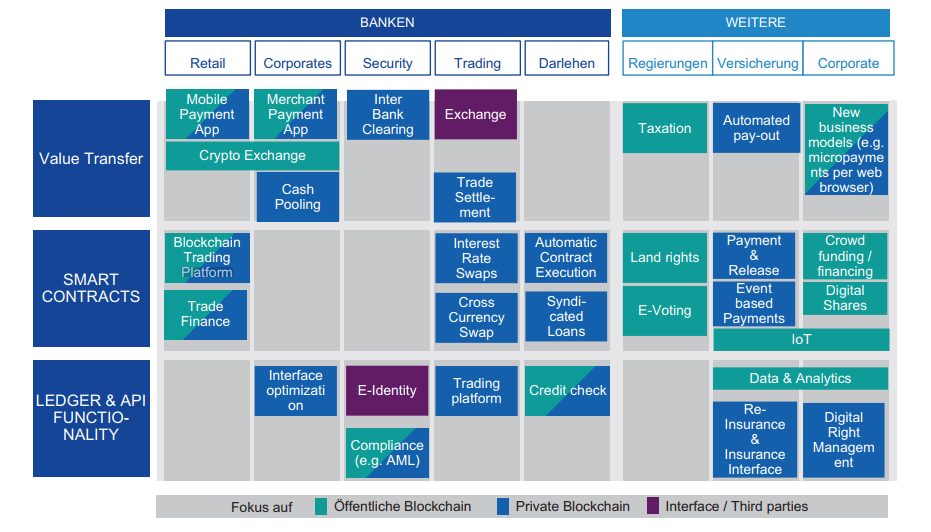
\includegraphics[width=1.0\textwidth]{gfx/blockchainanwendung.PNG}
 \caption{Korschinowski et al. \cite{Korschinowski2018}, S. 283, \enquote{Anwendungsfelder der Blockchain-Technologie. (Quelle: KPMG)}\label{fig:blockchain}}
\end{figure}

In Abb. \ref{fig:blockchain}, die Korschinowski et al. \cite{Korschinowski2018} übernommen haben wird ein Überblick der Anwendungsgebiete der \ac{DLT} gezeigt. In einigen Anwendungsbereichen hieraus könnten Ideen für zukünftige Plattformen nach der Vision von Goldman Sachs \ref{quote:goldman-vision} entstehen. Besonders in bankfachlichen Anwendungsgebieten müssen neue Technologien mit der Regulatorik abgewägt werden.

\paragraph{Idee: Software Development \enquote{as Code}}
\label{Disruption:DaaS}
Eine künftige Disruption würde möglicherweise als logische Folge auf die Auslagerung und Dematerialisierung fast aller Komponenten in der IT entstehen.
Es stellt sich die Frage ob der Entwickler oder die Entwicklungsarbeit selbst als eine vollautomatisierte Dienstleistung bereitgestellt werden kann. Dieses zukünftige Konzept könnte als Trend \enquote{Software Development as Code}\footnote{Im Rahmen der vollautomatisierten Bereitstellung von Entwicklerteams und Beratern} genannt werden, als Folge auf die neuen Rahmenbedingungen durch Cloud-Architekturen. Weiter Abstrahiert wird hierbei auch eine mögliche Vollautomatisierung von IT-Projektmanagement impliziert durch Orchestrierung der Einheiten.
Der Begriff \enquote{Software Development as a Service} existiert bereits im Rahmen einer Serviceorientierung der Entwicklung durch agile Methoden \cite{Lehman:2011}.

\emph{Freelancing} und \emph{Consulting} ist verbreitet in der IT und kann insbesondere aufgrund der zunehmenden Möglichkeiten und Akzeptanz für Remote-Arbeit sich immer weiter entwickeln. 

Dieses Konzept wäre aus Sicht der Innovationsförderung nicht negativ behaftet. Denn dadurch würden Zusammenarbeitsmodelle gefördert, die auf Offenheit, Agilität, Modularisierung und Kontinuität basieren und sich effektiv in den Ergebnissen auch zeigen und die Softwareentwicklung als solche optimieren.

Möglicherweise könnte nach einer Transformation der gesamten IT-Architektur hin zu einer Cloud-Architektur eine Disruption oder Diskontinuität entstehen mit unvorsehbaren Auswirkungen auf die IT. Cloud-Plattformen bieten eine Architektur, die allgegenwärtig und fortschrittlicher sein würde. Entwicklungs- und Produktivumgebungen werden weiterhin streng getrennt sein müssen \cite{MaRisk:2017}. Das ist jedoch kein Hindernis für neue Geschäftsmodelle in der Softwareentwicklung, so lange eine kontinuierliche Zusammenarbeit zwischen diesen Bereichen besteht.

Die Voraussetzungen aus regulatorischer Sicht wären die Rückverfolgbarkeit von Ergebnisartefakten im Softwareentwicklungsprozss, mithilfe von Automatisierung und Nachvollziehbarkeit der Delivery Pipeline und Risikomaßnahmen. Durch den Zugang einer Instanz der Entwicklungsumgebung gegenüber diesen Plattformen könnten Dienstleistungen für Entwicklungsarbeit analog zum Cloud-Computing gebucht werden.

Je nach Auslegung und Perspektive wäre diese beispielhafte Vorstellung eine Innovation oder Gefahr. Um ihr zu entgegnen sollte das Szenario durchgegangen werden. Für Entwickler entstehen möglicherweise Opportunitäten oder auch Risiken. 
\medskip
\\
Solche Entwicklungen werden unvermeidbar sein und zeigen sich zuerst in Form von Impulsen \cite{Bussmann2006} und nehmen mit zunehmender Reife der Technologie eine disruptive Eigenschaft an \cite{Ganswindt2006,Alt2017}. Die genannten Beispiele für disruptive und diskontinuierlichen Technologien zeigen, dass die Entwicklung keinen Halt macht und ständig gestalterisch fortgeführt werden kann und sich früher oder später materialisieren wird.

\section{Regulatorischer Rahmen für die IT im Finanzwesen}
Die \emph{Finanzkrise 2008} war mit einem enormen Vertrauensverlust gegenüber Banken verbunden und die Empörung der Gesellschaft ist durch das Internet und der daraus folgenden Transparenz viel größer als zuvor gewesen \cite{Eismann2015}. Eine Welle von regulatorischen Veränderungen als Folge auf die Auswirkungen dieser Krise herbeigeführt, um zukünftige systemische Krisen zu vermeiden \cite{Gupta:2017}. Das Ergebnis daraus ist ein Anstieg der regulatorischen Anforderungen mit gleichzeitiger Zunahme der technischen Anforderungen\footnote{insbesondere der \enquote{kontinuierliche Anstieg der Anforderungen an die IT-Architektur} \cite{Disterer2013}} in der IT. 

\begin{figure}[htbp]
 \centering
 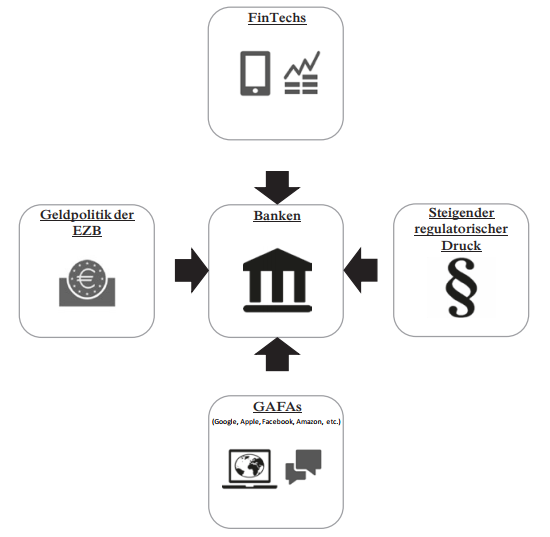
\includegraphics[width=0.8\textwidth]{gfx/bankdruck.PNG}
 \caption{\citet{Smolinski2017}, S. 44, Finanzbranche unter Druck}\label{fig:bankdruck}
\end{figure}

Daraus resultiert ein zunehmender Druck auf das Finanzwesen (Abb. \ref{fig:bankdruck}), der sich in wirtschaftlichem Druck und zusätzlichen Kosten zeigt \cite{Smolinski2017}.

\paragraph{BaFin Anforderungen}
Aus dem \ac{KWG} der Bundesrepublik Deutschland entstehen Anforderungen \cite{MaRisk:2017} an Kredit- und Finanzdienstleistungsinstitute, die sich auch auf die IT der Banken auswirken \cite{recht/Bornemann2018}. Im \ac{KWG} wird die BaFin für die Aufsicht der Institute nominiert \cite{recht/Bornemann2018}. Sie veröffentlicht Vorgaben an die von ihr beaufsichtigten Institute, um eine einheitliche Verwaltungspraxis sicherzustellen, mit der sich die Institute auf die Prüfungen der BaFin einstellen \cite{BaFin:Verwaltungspraxis}. 

Die BaFin präzisiert in \cite{MaRisk:2017} die Anforderungen des \ac{KWG} im Bereich Risikomanagement und Auslagerung. In \cite{BAIT:2018} werden diese Anforderungen für den Bereich der IT nochmals konkretisiert. Hierdurch sollen operationelle Risiken auch in der IT angemessen gesteuert werden. \citet{mci/Knittl2013} beschreibt die Umsetzung dieser Anforderungen anhand einer Fallstudie zu einem internationalen Finanzkonzern.
\medskip
\\
\paragraph{Finanzwesen unter Druck}
Abb. \ref{fig:bankdruck} verbildlicht, wie Banken von allen Seiten unter Druck stehen. Die Darstellung könnte fortgeführt werden mit der Annahme, dass die äußeren Kräfte sich auch gegenseitig beeinflussen. Die Technologien und Trends aus den \enquote{GAFAs} können mit Sicherheit als ein Antreiber für die FinTechs gesehen werden. Die Antreiber von Veränderung auf der vertikalen Achse der Abbildung werden von Einschränkenden Instituten auf der horizontalen Achse durchkreuzt. Die Aufsichten evaluieren ebenfalls neue Technologien und berücksichtigen sie jeweils bei der Novellierung ihrer Rahmenwerke \cite{BaFin:marisk-novelle}. Bis diese angepasst werden vergeht Zeit und bis sich die etablierten Institute hierauf auch anpassen vergeht ebenfalls wertvolle Zeit. In FinTechs ist dieses Problem aufgrund ihrer Agilität und Effizienz geringer. Etablierte Institute müssen daher einen Weg finden das Zusammenspiel zwischen neuen Technologien und regulatorischen Anforderungen zu antizipieren und eigene Initiativen als Pilotprojekte schon zu starten. Hierzu passt ebenfalls der Ansatz der Vorwegnahme durch die Gestaltung von Zukunftszuständen \cite{Alt2017}.


\paragraph{Ermessen der Institute}
\label{ermessensfreiheit}
In \cite{MaRisk:2017, BAIT:2018} fällt auf, dass viele Vorgaben durch entsprechende Wörter in ihrem Gewicht relativiert werden. Die Maßnahmen zu ihrer Umsetzung liegen hierbei im Ermessen der jeweiligen Institute. Im Interesse der Institute ist in erster Linie das Bestehen von Prüfungen der Aufsicht. Die Ermessensfreiheit könnte in einigen Bereichen für Unklarheit sorgen, da die \ac{MaRisk} sehr abstrakt formuliert ist \cite{DSGV:2019}.
Eine Kultur innerhalb der internen Kontrollverfahren die sich nur auf Umsetzung beschränkt zum bestehen von Prüfungen sollte als Folge vermieden werden. Eine Mitgestaltung ist hierbei wichtig um eine gemeinsame Wissensplattform aufzubauen. \citet{DSGV:2019} hat einen gemeinsamen Leitfaden gestaltet, dass selbst in Papierform eine Plattform darstellt. Selbst gemeinsame Wissensplattformen könnten einen ersten Beitrag zur Innovationskraft sein und somit als Anlage gesehen werden. Der antreibende Faktor dahiner wäre die Kommunikation und Schnittstellen. Die Voraussetzung hierfür wäre Offenheit.

Die Flexibilität, die die \ac{BaFin} in ihren Rahmenwerken vorsieht \cite{MaRisk:2017} sollte als stärke wahrgenommen werden und auf die interne Kultur übertragen werden. Die internen Kontrollverfahren und das Risikomanagement müssen in erster Linie praxisnah und flexibel bezüglich der IT vorgehen und ihren Ermessensspielraum zu Nutze machen, um mit neuen Technologien umgehen zu können. Die Ermessensfreiheit, die die \ac{BaFin} beschreibt erzeugt nur Druck und Unsicherheit in Instituten, denen es an Gestaltungsfähigkeit fehlt. Die \ac{BaFin} verlangt mit der IT-Strategie \cite{BAIT:2018} ein aktives Mitgestalten seitens Management. Ebenso sieht sie genug Gestaltungsfreiheit für das Risikomanagement vor. Daher sollte das Risikomanagement und das \ac{ITM} diesen Ansatz sich aneignen. Banken sind zugegebenermaßen auf Profitmaximierung angewiesen. 

Für die \ac{MaRisk} gibt es auch zusätzliche Erläuterungen der BaFin \cite{MaRiskErläuterungen:2017}. Speziell für die IT hat die BaFin in \cite{BAIT:2018} die \ac{MaRisk} noch einmal konkretisiert. Daneben gibt es institutspezifische Interpretationen und Werke \cite{DSGV:2019}.

\paragraph{Risikomanagement}
Für das Risikomanagement fordert die \ac{BaFin} die Festlegung von Strategien und die Einrichtung von internen Kontrollverfahren, bestehend aus einem \ac{IKS} und einer interne Revision. Ein Risikomanagement für die IT soll insbesondere den Betrieb schützen \cite{MaRisk:2017}, da hierin die operationellen Risiken liegen. 

Ein Ausfall der IT-Systeme in Banken hätte mit Sicherheit Auswirkungen auf kritische Geschäftsprozesse, die bis hin zu einer systemischen Krise führen könnten.

Daher fordert die \ac{BaFin} \cite{MaRisk:2017} vom IT-Risikomanagement:
\begin{enumerate}
    \item Sie soll Überwachungs- und Steuerungsprozesse für IT-Risiken einrichten.
    \item Ihre Prozesse umfassen: Risikokriterien, Risiken, Schutzbedarf, Schutzmaßnahmen, Risikobehandlung und -minderung
    \item Sie soll Risiken beim Einkauf von Software \emph{angemessen} bewerten.
\end{enumerate}
Diese Forderungen \cite{MaRisk:2017} zur Bewertung von IT-Risiken gelten auch beim Einsatz von selbst entwickelten Anwendungen, die von ihr als \ac{IDV} bezeichnet wird. Entsprechende Maßnahmen sollen jedoch nach dem Schutzbedarf der unterstützten Prozesse und verarbeiteten Daten festgelegt werden \cite{MaRisk:2017}.

Die Überwachungs- und Steuerungsprozesse für IT-Risiken sollten daher klare Grenzen für die Verarbeitung von Daten definieren. Eine klare Unterscheidung zwischen \ac{IDV} Anwendungen und Anwendungen die keine \ac{IDV} darstellen ist nötig, um angemessene Maßnahmen festzulegen. Da \ac{IDV} Anwendungen jedoch hierbei pauschalisiert gesehen werden und aufgrund der darauf folgenden aufwendigen Maßnahmen negativ behaftet sind wird ihre Katalogisierung entmutig. Somit entsteht oft eine \enquote{Schatten-IT} in Banken \cite{Dorschel2018}.

Die Ermessensfreiheit zu den Maßnahmen des Risikomanagements begrenzt sich in diesem Fall auf den Schutzbedarf der Geschäftsprozesse und Daten. Daher muss die Katalogisierung von Anwendungen bezüglich ihres Schutzbedarfs in einem Spektrum ausgeweitet. Es kommt darauf an welche Daten von der Anwendung verarbeitet werden. Dieser Punkt sollte nachvollziehbar zu den Anwendungen dokumentiert werden.

\paragraph{IT-Systeme und Prozesse}
Die \ac{BaFin} \cite{MaRisk:2017} fordert zu IT-Systemen und Prozessen:
\begin{enumerate}
    \item IT-Systeme und Prozesse sollen Integrität, Verfügbarkeit, Authentizität und Vertraulichkeit der Daten mit gängigen Standards sicherstellen.
    \item IT-Systeme und ihre zugehörigen Prozesse sollen hinsichtlich ihrer Eignung regelmäßig überprüft werden.
    \item IT-Systeme sollen nach \emph{wesentlichen} Veränderungen und vor erstmaligem Einsatz getestet werden.
    \item Ein Regelprozesse der Entwicklung, des Testens, der Freigabe und der Implementierung in die Produktionsprozesse soll etabliert werden. 
    \item Produktions- und Testumgebungen sollen grundsätzlich voneinander getrennt werden.
\end{enumerate}
%
Besonders hervorzuheben ist die Verantwortung der IT-Systeme und Prozesse für die Sicherstellung der Datensicherheit. Im Fokus stehen die verarbeiteten und gespeicherten Daten in den IT-Systemen und Prozessen. 

Hierzu fordert die BaFin \cite{MaRisk:2017} eine Orientierung am Schutzbedarf der verarbeiteten Daten. Sie verweist mit gängigen Standards auf den IT-Grundschutzkatalog\footnote{vgl. IT-Grundschutzkompendium \cite{IT-Grundschutz:2020}} des \ac{BSI} und auf den internationalen Sicherheitsstandard ISO/IEC 2700X\footnote{vgl. Disterer \cite{Disterer2013}} der \ac{ISO}.

Die Auslagerung von IT-Ressourcen wäre beispielsweise bei der Entwicklung von Modellen für Mashinelles-Lernen nötig und dürfte aufgrund der Datensicherheit nicht ohne weiteres auf einer externe Cloud-Plattform durchgeführt werden. 
\medskip
\\
Auch im Bereich der Automatisierung von Prozessen ist es wichtig zu erkennen, welche unterstützten Prozesse schutzbedürftig sind und welche nicht. IT-Prozesse können grob zwischen \emph{Change} und \emph{Run} unterteilt werden \cite{Dorschel2018}. Die Run-Prozesse regeln den Betrieb und die Change-Prozesse erzeugen üblicherweise als Projektform Veränderungen im Aufbau oder Ablauf der Organisation.

Die Softwareentwicklung selbst enthält innerhalb einer getrennten Testumgebung auf dem ersten Blick keine operationellen Risiken für den Geschäftsbetrieb der Bank. Für die Integrierung von Ergebnissen aus diesen Change-Prozessen in den Betrieb ist eine vorherige Freigabe vorgesehen, beispielsweise in Form von \enquote{Quality-Gates} \cite{mci/Disterer2011}.

Für ihre Unterstützung existiert innerhalb der IT ein eigener Betrieb für Plattformen und Anwendungen der Softwareentwicklung. Ein hoher Schutzbedarf der Entwicklung entsteht in Folge von Schnittstellen bedingt durch Prozesse für die Inbetriebnahme von Software. Besonders ist in der Anwendung von DevOps die Delivery-Pipeline, womit die Komponenten in die Produktionsumgebung integriert werden ein kritischer Prozess. Nach DevOps sind die Abläufe zwischen \ac{CI} und \ac{CD} für einen automatisierten und hochfrequenten Ablauf eng miteinander verbunden. In \ac{CD} liegt auch die Verantwortung über Risiken und Qualitätssicherung \cite{Alt2017}.
Es stellt sich die Frage wie Anwendungen zur Ausführung der Delivery Pipeline bezüglich ihres Schutzbedarfs einzuordnen sind. 

\paragraph{Konsequenzen für die SEU}
Grenzen zeigen sich zum Beispiel in Form von unterschiedlichen Zonen innerhalb der IT-Architektur. 
Diese Grenzen sind nötig, um die Risiken für den Betrieb kontrollieren zu können. Hierfür wird eine klare Nachvollziehbarkeit der Ergebnisse aus den Change-Prozessen bedingt.

Innerhalb der \ac{SEU} sind die Rollen schwierig voneinander zu unterscheiden. Konfiguration, Administration, Wartung und Weiterentwicklung von Anwendungen für die \ac{SEU} sind Tätigkeiten in denen Kunde, Entwickler und Betrieb (Abb. \ref{fig:devops}) teilweise ineinander verschmelzen. Auch die technische Umsetzung der Überwachungsprozesse erfolgt meist von den gleichen Entwicklern der \ac{SEU}. 
Die enge Kopplung zwischen Entwicklung und Betrieb ist in DevOps vorgesehen \cite{} und setzt agile und kontinuierliche Prinzipien voraus, die aus Sicht des Risikomanagements schwierig zu kontrollieren sein könnten. 

Die Auslagerung der \ac{SEU} auf externe Infrastrukturen ist aufgrund dieser engen Kopplung der Abläufe in DevOps beschränkt, weil hierdurch sensible Daten ausgetauscht werden könnten. Zudem könnte eine zu hohe Abhängigkeit zu einer Cloud-Plattform für den Betrieb der \ac{SEU} entstehen. Realistischer wäre es bei Bedarf nur einzelne rechenintensive Services auszulagern mit Ansätzen für eine hybride Cloud \cite{Gupta:2017}. 

Selbst wenn diese Modularisierung mit neuen Technologien wie Container-Virtualisierung realisierbar ist, bestehen für die Verwendung von externen Cloud-Plattformen Probleme bezüglich der Datensicherheit. 

\paragraph{Wesentliche Veränderungen}
Bei wesentlichen Veränderungen (\emph{Change-Prozesse}) bedingt die \ac{BaFin} \cite{MaRisk:2017} vom Risikomanagement die Auswirkung der Veränderung auf die Kontrollverfahren zu analysieren. Hierfür sind die später in die Arbeitsabläufe eingebundenen Organisationseinheiten, Risikocontrolling, Compliance und die Interne Revision zu beteiligen. 
\medskip
\\
Daraus könnte ein Hindernis für solche Veränderungen entstehen. Wesentliche Veränderungen in den IT-Systemen könnten einen Anpassungsbedarf des Kontrollverfahrens bedeuten. Vielmehr sollte das interne Kontrollverfahren von einer ständigen Veränderung in der IT ausgehen und sich auf Auswirkungen vorbereiten.

\paragraph{Bankaufsichtliche Anforderungen an die IT}
Die \ac{BAIT} gibt seit 2018 neben der \ac{MaRisk} auf der gleichen Grundlage des \ac{KWG} einen  Rahmen, insbesondere für das Management der IT-Ressourcen und das IT-Risikomanagement. Die Anforderungen aus \ac{MaRisk} werden lediglich konkretisiert. Zudem Präzisiert es die Anforderungen des § 25b des
\ac{KWG} zu Auslagerung von Aktivitäten und Prozessen \cite{BAIT:2018}.
\\
Die \ac{BAIT} ist daher besonders für die Auslagerung von IT-Ressourcen zu berücksichtigen und insbesondere aufgrund der zunehmenden Praxis von \ac{SaaS} und Cloud-Computing relevant.

\paragraph{IT-Strategie} Die Geschäftsleitung soll eine nachhaltige IT-Strategie festlegen, die konsistent mit der Geschäftsstrategie ist \cite{BAIT:2018}. 

Aus den Mindestinhalten der geforderten IT-Strategie wird deutlich, dass Geschäftsmodell und IT in einem engen Verhältnis gesehen werden. Die IT steht aus regulatorischer Sicht nicht mehr größtenteils als Risikofaktor im Fokus. Vielmehr kann sie aufgrund einer konkreten Strategie das Geschäftsmodell ergänzen. Diese Anforderung ist eine klare Förderung der Rolle der IT. 

\paragraph{IT-Governance} Die IT-Governance wird als Struktur zur Steuerung und Überwachung des IT-Betriebs und der Entwicklung der IT-Systeme und Prozesse auf Basis der IT-Strategie \cite{BAIT:2018} gesehen. Für das Risikomanagement, Entwicklung und Betrieb innerhalb der IT wird eine qualitativ und quantitativ angemessene Ausstattung mit Personal gefordert.

\paragraph{EBA Guidelines}
Bedeutende Institute werden zusätzlich von der \ac{EBA} beaufsichtigt \cite{recht/Bornemann2018}. Die \ac{EBA} veröffentlicht für sie eine Richtlinie \cite{eba:2019}, die sich auf die \ac{MaRisk} bezieht und für die systemrelevanteren Institute wichtig sind.

\paragraph{Idee für ein innovatives Risikomanagement}
Die von \citet{mci/Disterer2011} beschriebenen Probleme im Betrieb von Anwendungen durch die mangelnde Beachtung von nichtfunktionalen Anforderungen und die Einführung von Quality Gates könnten hierbei auf Probleme für die internen Kontrollverfahren ausgeweitet werden. 
\medskip
\\
Eine Koordination zwischen Entwicklung und Betrieb sollte das IT-Risikomanagement miteinbeziehen. Dabei sollte die Geschwindigkeit des Entwicklungs- oder Integrationsprozesses nicht beeinträchtigt werden. Hierfür sollte das IT-Risikomanagement agile Methoden verwenden. Die Schnelligkeit hat bei der Beantwortung von Compliancefragen dabei eine wichtige Rolle. Entwickler könnten zuerst die Prozesse des IT-Risikomanagements optimieren und automatisieren, um sich Handlungsfreiheit für Innovation und wesentlichen Veränderungen innerhalb der Organisation zu schaffen. Sie sollten in das Risikomanagement integriert werden. Ein Entwickler aus einem anderen Projekt könnte als Compliance- und Risikoverantwortlicher parallel wichtige Compliancefragen auf technischer Ebene schnell überprüfen und vorab beantworten. Dadurch könnte unter Vorbehalt schon mit neuen Technologien und Methoden an Lösungen gearbeitet werden oder Veränderungen in Gang gesetzt werden. 

Um einer Disruption zu begegnen ist das Risiko von verschwendetem Aufwand in Kauf zu nehmen, um sich eine Anpassungs- und Reaktionsfähigkeit zu schaffen, die geschäftskritisch ist \cite{Bussmann2006}.

\subsection{Paradigmawechsel der Regulatorik}

\paragraph{Relevanz der Regulatorik für Entwickler}
Die BaFin Anforderungen \cite{MaRisk:2017, BAIT:2018}, Gängige Sicherheitsstandards \cite{IT-Grundschutz:2020, Disterer2013} und weitere Rahmen sind für Entwickler wichtig, um ihre Verantwortung über die IT-Risiken in Banken und anderen systemrelevanten Betrieben zu verstehen. Insbesondere sind sie für die nachvollziehbarer Entwicklung von Anwendungen und Systemen und für ihren nachhaltigen Betrieb, Überwachung und Überprüfung zu berücksichtigen. Um verwachsene und unflexible Architekturen zu vermeiden sollten Entwickler, im Bereich der Anwendungen, die interne Prozesse unterstützen \cite{Bussmann2006}, sich mit diesem Thema auseinandersetzen.
\medskip
\\
Neben den Leistungsansprüchen sollten die Sicherheitsansprüche für Veränderungen im Vordergrund stehen. Die Implementierung von neuen Technologien wirft bei wesentlichen Veränderungen viele Compliancefragen auf \cite{MaRisk:2017}. Diese hängen mit den Sicherheitsansprüchen zusammen und sind unvermeidbar, können aber durch eine Effizienzsteigerung der Steuerungs- und Überwachungsprozesse zu einer Stärke werden und die Fähigkeit wesentliche Veränderungen durchzuführen erhöhen
\medskip
\\
Aufgrund befürchteten aufwändigen Maßnahmen sollte die Durchführung von wesentlichen Veränderungen nicht entmutigt werden. Die Maßnahmen fokussieren sich den Schutzbedarf von kritischen Prozessen und Daten (Kap. \ref{ermessensfreiheit}). Es wäre daher eine Selbstbeschränkung die Maßnahmen aufgrund eines mangelnden Verständnisses der Regulatorik zu pauschalisieren, somit die Ermessensfreiheit aufzugeben und präzisere Vorgaben von der Aufsicht zu fordern.

Ein \enquote{Schwarz-Weiß} Denken als Folge zum Bestehen von Prüfungen oder die Umsetzung des Trugschlusses \enquote{Security through Obscurity} sind zu vermeiden. Das Pauschalisieren der geforderten Maßnahmen des Risikomanagement könnte eine \enquote{Schatten-IT} \cite[S. 104]{Dorschel2018} erzeugen, aufgrund ihrer Befürchtungen. 
\medskip
\\
Ein Beispiel wäre die Katalogisierung von \ac{IDV} Anwendungen \cite{BAIT:2018}, \cite[Kap. 6.8]{Dorschel2018}. Ein mangelndes Verständnis über die Hintergründe der Forderungen würde sich in einer mangelnden Selbsteinschätzung der Maßnahmen zeigen. Dies hätte zu Folge, dass Entwickler aufgrund ihrer Befürchtungen gegenüber den Maßnahmen die Kommunikation und somit Offenheit gegenüber des Risikomanagements und \ac{ITM} einschränken.
%
\subsection{Aufsicht und IT-Strategie}
Bezüglich des Finanzwesens befindet sich möglicherweise auch die deutsche Verwaltungspraxis im Wandel. Insbesondere hat die Cloud-Technologie neue Impulse für das Thema \emph{Auslagerung von IT-Ressourcen \cite{MaRisk:2017, BAIT:2018}} erzeugt. Die \ac{MaRisk} wird voraussichtlich 2021 erneuert und darüber hinaus sind Erleichterungen aufgrund der Umsetzung der EBA-Richtlinien \cite{eba:2019}\footnote{seit 30. Juni 2020 in kraft getreten} zu erwarten \cite{BaFin:marisk-novelle}. 
\medskip
\\
Die Anpassung der Verwaltungspraxis kommt jedoch gezwungenermaßen und konnte dem Veränderungsdruck der Institute (Abb. \ref{fig:bankdruck}) nicht standhalten. Die Aufsicht und ihre beaufsichtigten Institute sollten sich einen Weg überlegen, wie Veränderungen kontinuierlich stattfinden können, wie sie \citet{Bussmann2006} fordern.
\medskip
\\
Im Gegensatz zur \ac{MaRisk} nimmt die \ac{EBA} im Anhang ihrer Richtlinie \cite{eba:2019} Stellung zum Thema Innovation, Transformation und IT-Strategie und geht dabei auf Kommentare und Fragen zu ihrer Richtlinie zusammen.
\medskip
\\
Die \ac{EBA} fasst den Vorschlag eines Korespondenten zusammen \cite[S. 50]{eba:2019}:
\begin{quote}
    \enquote{
Der Text
\footnote{Bezogen auf \emph{Guidelines on ICT and security risk
management
} \cite[S. 14ff]{eba:2019}} 
sollte auch die Ausrichtung der IKT-Strategie\footnote{\ac{IKT} -Strategie übersetzt von \enquote{ICT-Strategy}} nach Innovation enthalten, zur Vermeidung von Disruption und zur Unterstützung schlanker digitaler Transformation, die auf \ac{IKT}-Architektur basiert. Es\footnote{Die Richtlinie} sollte auch das richtige Portfolio von Änderungen enthalten, zur Ausrichtung der \ac{IKT}-Transformation in Einklang mit Geschäftstransformation.
    }\footnote{Übersetzt aus dem Englischen, Respondent unbekannt}
\end{quote}

Die Sorgen der Beteiligten zu disruptiven Verläufen \cite{Ganswindt2006, Alt2017} von Technologiesprüngen und der damit zusammenhänge Aufwand eine Transformation der Architektur durchzuführen wird hierbei deutlich. Hierbei ist auch von richtigem Portfoliomanagement die Rede, um für die richtigen Änderungen zu priorisieren.

Die Antwort der \ac{EBA} hierauf verweist auf die IT-Strategie, die Teil der Gesamtstrategie ist \cite[S. 14ff]{eba:2019}. Somit stehen Banken in der Eigenverantwortung sich eine Strategie für disruptive Technologiespürnge zu erarbeiten.